\usepackage[utf8]{inputenc}
\usepackage[T1]{fontenc}

\usepackage[a4paper]{geometry}
\geometry{
  a4paper,
  left=25mm,
  right=25mm,
  top=25mm,
  bottom=25mm
}
% title 
\makeatletter
\renewcommand\maketitle{
  {
      \vspace*{3cm}
      \raggedright % Note the extra {
      \begin{center}
        {\normalsize \sffamily \course }\\[2ex]
        {\Large \bfseries \sffamily \@title }\\[2ex]
        {\normalsize  \@author}\\[1ex]
        \@date\\[4ex]
      \end{center}
      \vspace*{1cm}
      \begin{center}
        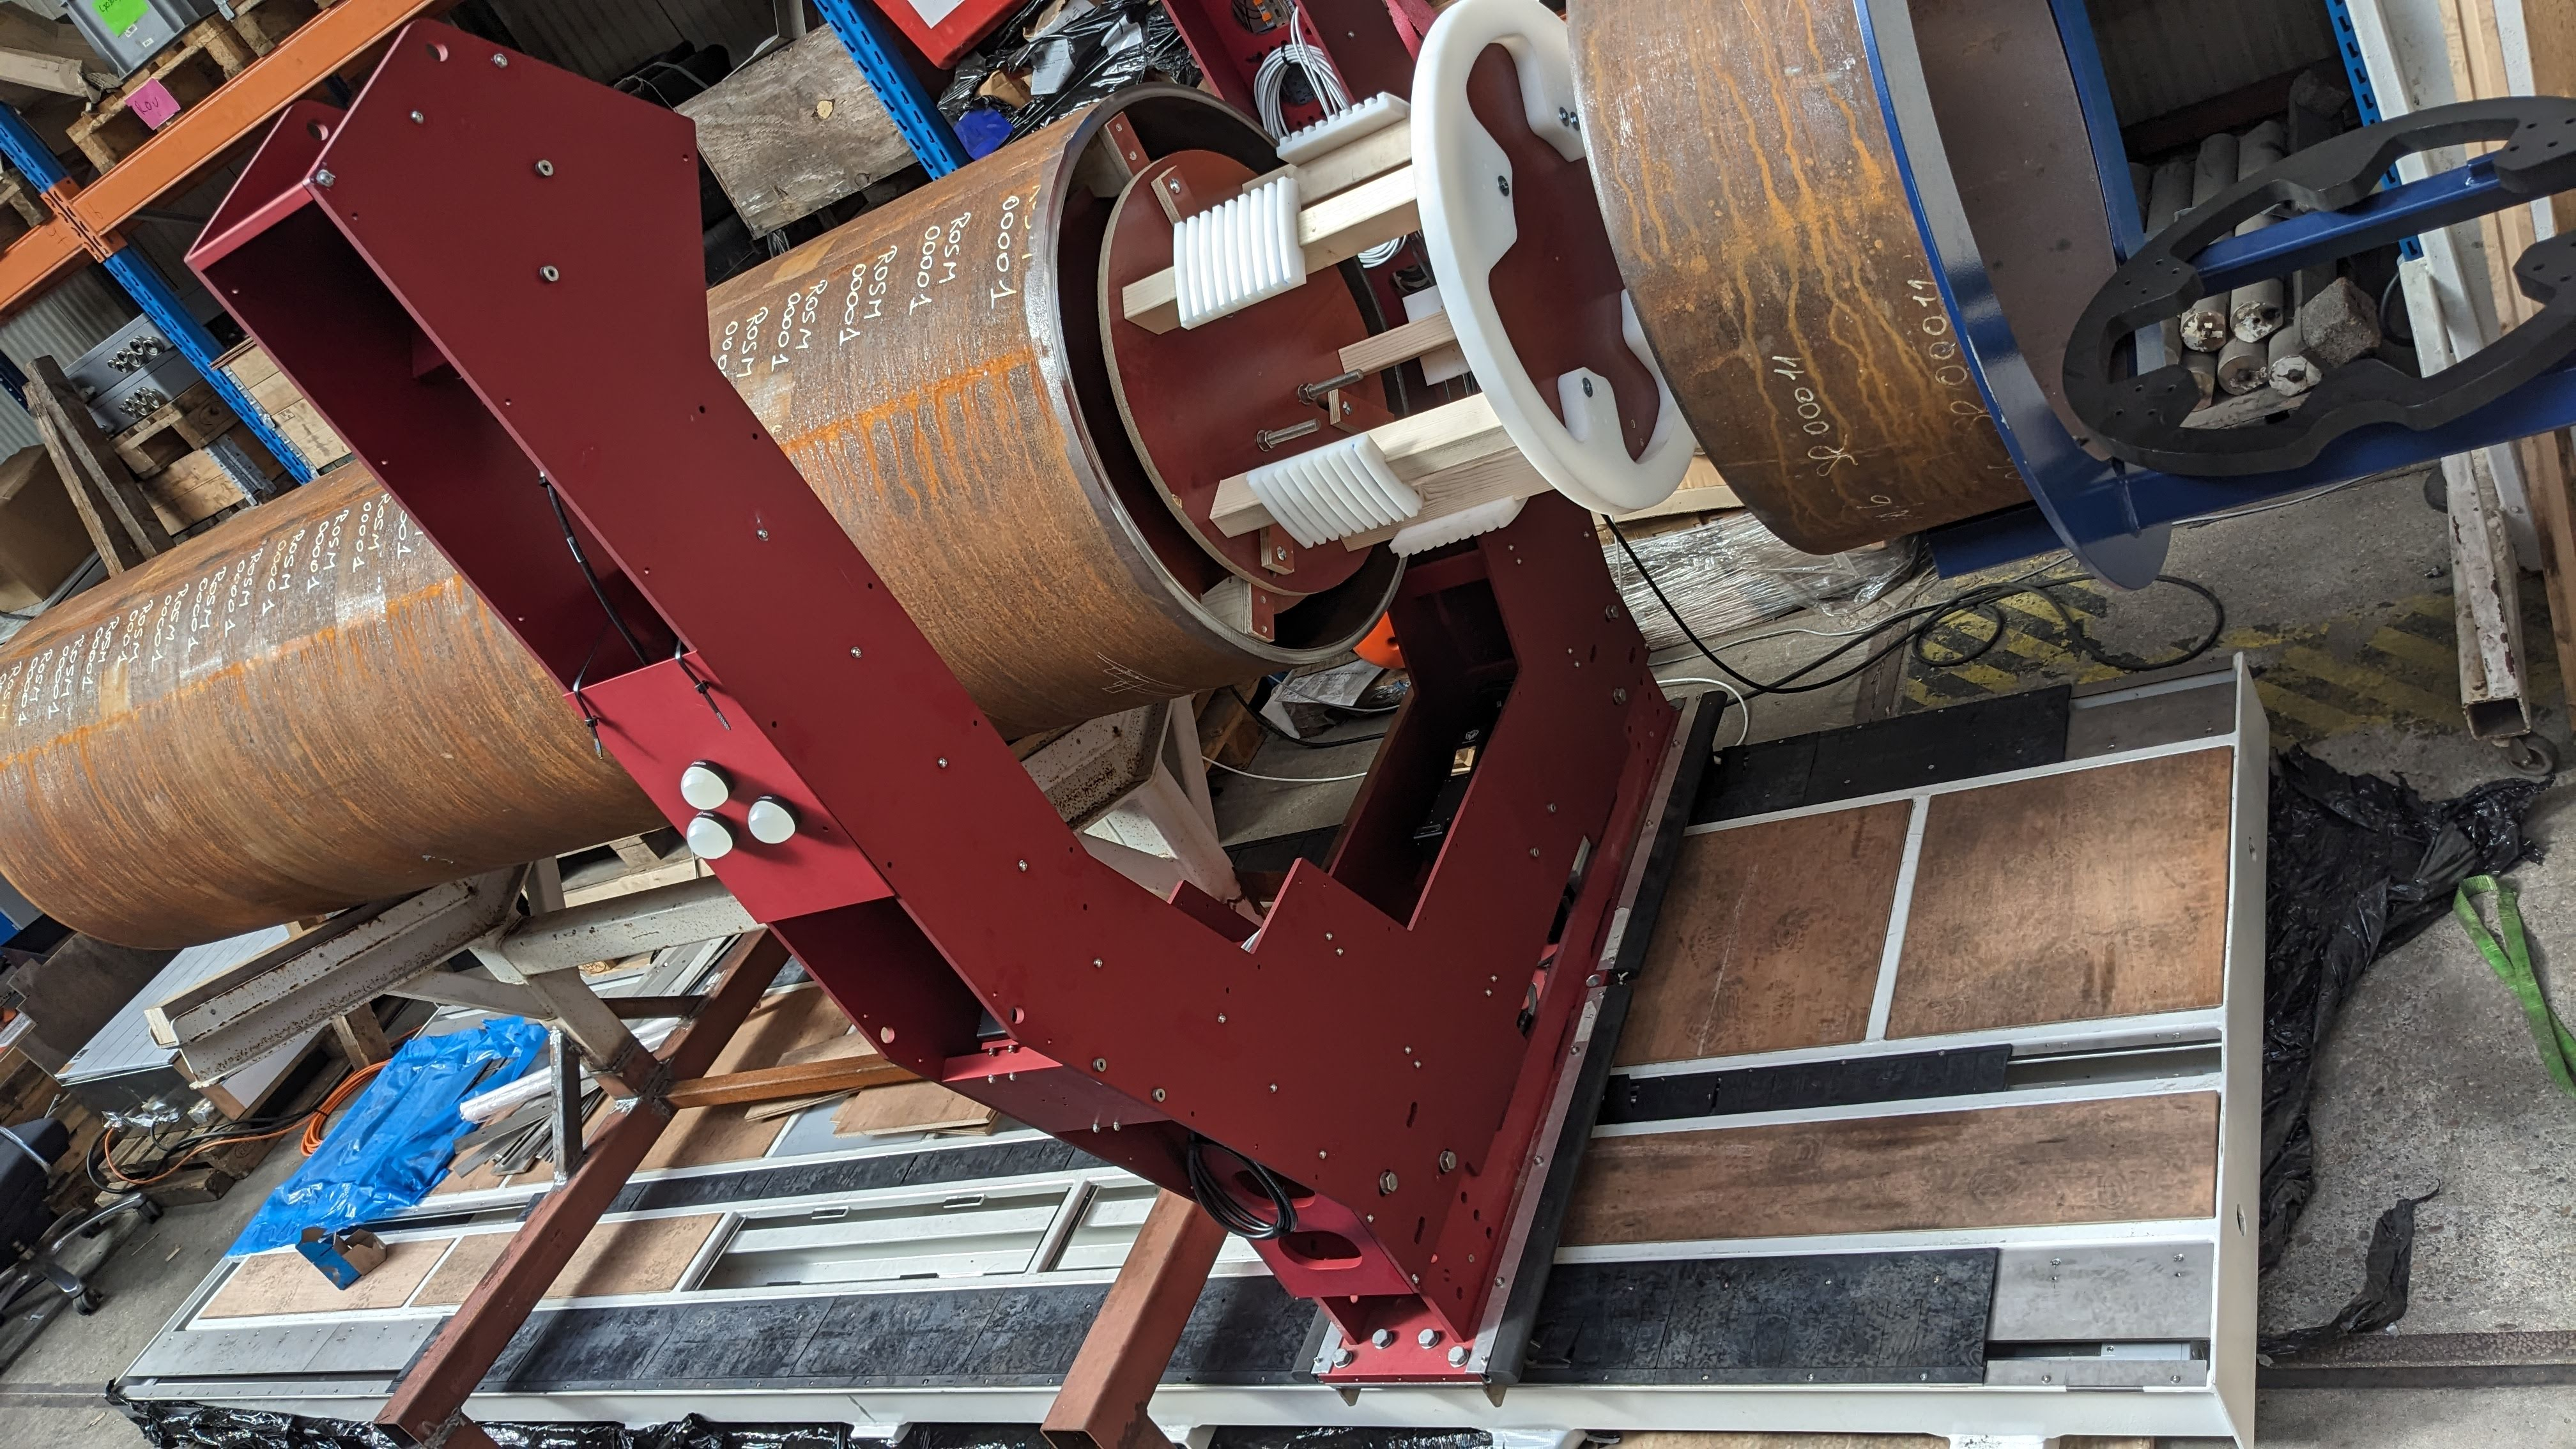
\includegraphics[width=0.5\textwidth]{images/cover.jpg}
      \end{center}
    }

    % TUD logo
    {
      \begin{tikzpicture}[remember picture, overlay]
        \node[anchor=north west, inner sep=40pt] at (current page.north west)
        {
\includegraphics[width=0.3\textwidth]{images/logo_TUD.png}};
      \end{tikzpicture}
    }

    % Allseas logo
    {
      \begin{tikzpicture}[remember picture, overlay]
        \node[anchor=north east, inner sep=40pt] at (current page.north east)
        {
\includegraphics[width=0.3\textwidth]{images/logo_Allseas.png}};
      \end{tikzpicture}
    }

    % uni supervisor info text (bottom left)
    {
      \begin{tikzpicture}[remember picture, overlay]
        \node[anchor=south west, inner sep=40pt] at (current page.south west)
        {
          \begin{minipage}{0.5\textwidth}
            \small
            \textbf{University supervisor:} \\
            \nameunisupervisor \\
            \university \\
            \faculty
          \end{minipage}
        };
      \end{tikzpicture}
    }

    % company supervisor info text (bottom left)
    {
      \begin{tikzpicture}[remember picture, overlay]
        \node[anchor=south east, inner sep=40pt] at (current page.south east)
        {
          \begin{minipage}{0.5\textwidth}
            \small
            \begin{flushright}
              \textbf{Company supervisor:} \\
              \namecompsupervisor \\
              \role \\
              \department
            \end{flushright}
          \end{minipage}

        };
      \end{tikzpicture}
    }
}
\makeatother

% Multiple columns
\usepackage{multicol}

% Better fonts
\usepackage{newpxtext}

% Removes indentation and adds vspace
% \usepackage{parskip}

% Equations and mathematical symbols
\usepackage{amsmath, amssymb, amsthm}
\usepackage{mathtools} % ?

% Images and captions
\usepackage{graphicx}
\usepackage[font=small,labelfont=bf]{caption}
\usepackage{float}

% Appendices
\usepackage{appendix}

% Code listings
\usepackage{listings}
\usepackage[dvipsnames]{xcolor}
\usepackage{transparent}
\lstset{frame=tb,
  language=Python,
  aboveskip=7mm,
  belowskip=7mm,
  columns=flexible,
  basicstyle={\footnotesize\ttfamily},
  keywordstyle={\bfseries\color{NavyBlue}},
  commentstyle=\color{Gray},
  stringstyle=\color{Green},
  breaklines=false,
  breakatwhitespace=true,
  tabsize=3,
  morecomment=[l][\color{Gray}\transparent{0.5}]{\#},
}


\usepackage{algorithm}
\usepackage{algpseudocode}


%%%%%%%%%%%%%%%%%
% Custom macros %
%%%%%%%%%%%%%%%%%


% Probability measure
\renewcommand{\P}{\mathbb{P}}

% Expectation
\newcommand{\E}{\mathbb{E}}

% (*) above a symbol
\newcommand\mygt{\stackrel{\mathclap{\scriptsize\mbox{$(\ast)$}}}{>}}



% theorems
\usepackage{tikz}
\usepackage{tikz-cd}
\usepackage{thmtools}
\usepackage[framemethod=TikZ]{mdframed}
\mdfsetup{skipabove=1em, skipbelow=1em, innertopmargin=5pt, innerbottommargin=6pt}

\theoremstyle{definition}

\makeatletter


\declaretheoremstyle[headfont=\bfseries\sffamily, bodyfont=\normalfont, numbered=no, mdframed={nobreak}]{problembox}

\declaretheoremstyle[headfont=\bfseries\sffamily, bodyfont=\normalfont, mdframed={}]{thmbox}
\declaretheoremstyle[headfont=\bfseries\sffamily, bodyfont=\normalfont, numbered=no, mdframed={ rightline=false, topline=false, bottomline=false, }, qed=\qedsymbol ]{proofbox}
\declaretheoremstyle[headfont=\bfseries\sffamily, bodyfont=\normalfont, numbered=no, mdframed={ nobreak, rightline=false, topline=false, bottomline=false}]{infobox}

\declaretheorem[style=problembox, name=Problem Definition]{problem}
\declaretheorem[style=problembox, name=Weak Form]{weakform}
\declaretheorem[style=infobox, name=Assumption]{assumption}

\declaretheorem[style=thmbox, name=Definition]{definition}
\declaretheorem[sibling=definition, style=thmbox, name=Corollary]{corollary}
\declaretheorem[sibling=definition, style=thmbox, name=Proposition]{prop}
\declaretheorem[sibling=definition, style=thmbox, name=Theorem]{theorem}
\declaretheorem[sibling=definition, style=thmbox, name=Lemma]{lemma}

\declaretheorem[style=proofbox, name=Proof]{boxedproof}
\declaretheorem[style=infobox, name=Explanation]{explanation}
\declaretheorem[style=infobox, name=Exercise]{ex}
\declaretheorem[style=infobox, name=Example]{eg}
\declaretheorem[style=infobox, name=Remark]{remark}
\declaretheorem[style=infobox, name=Note]{note}


\declaretheoremstyle[headfont=\bfseries\sffamily, bodyfont=\normalfont, numbered=no, mdframed={} ]{thmsolutionbox}
\declaretheorem[numbered=no, style=thmsolutionbox, name=Solution]{solution}


\newif\ifshowcomments
\showcommentstrue
% \showcommentsfalse
\ifshowcomments
  \newcommand{\mynote}[2]{\fbox{\bfseries\sffamily\scriptsize{#1}}
    {\small$\blacktriangleright$\textsf{\emph{#2}}$\blacktriangleleft$}}
  \newcommand{\citehere}[0]{\textcolor{red}{\fbox{\bfseries\sffamily\scriptsize{CITATION}}}}
\else
  \newcommand{\mynote}[2]{}
  \newcommand{\citehere}[0]{}
\fi
\newcommand{\todo}[1]{\textcolor{blue}{\mynote{To do}{#1}}}

% Bibliography
\usepackage[backend=biber, style=apa, citestyle=numeric-comp]{biblatex}
\addbibresource[type=file, glob,datatype=bibtex,location=local]{bibliograhy.bib}
\DeclareFieldFormat{url}{\href{#1}{\mkbibacro{URL}}} % URL's clickable

% Hyperlinks
\usepackage{hyperref}
\hypersetup{
  colorlinks=true,
  linkcolor=blue,
  filecolor=magenta,
  urlcolor=blue,
  citecolor=blue,
  pdftitle={Overleaf Example},
  pdfpagemode=FullScreen,
}

\urlstyle{same}
\usepackage{cleveref}

\usepackage{subcaption}
% \usepackage{subfig}

% symbols
\usepackage{twemojis}